%%=============================================================================
%% Gebruikersonderzoek
%%=============================================================================

\chapter{Gebruikersonderzoek}
\label{ch:gebruikersonderzoek}

\section{Inleiding}

De enquête werd volledig anoniem afgenomen.


\section{Resultaten en analyse}

In de volgende secties zullen de resultaten van de enquête besproken en geanalyseerd worden.

\subsection{Demografie}

\textbf{Resultaat}

De grootte van de steekproef bedraagt 66 deelnemers. De verdeling van deze deelnemers volgens hun geslacht en leeftijden wordt weergegeven in de Tabellen \ref{tab:verdelinggeslacht} en \ref{tab:verdelingleeftijden}. In tabel \ref{tab:verdelinggeslacht} is te zien dat de steekproef uit iets meer vrouwen (57,6\%) dan mannen (42,4\%) bestaat. Tabel \ref{tab:verdelingleeftijden} toont dat de deelnemers werden onderverdeeld op basis van hun leeftijd in zeven categorieën. Hieruit is op te maken dat de leeftijden varieerden van jonger dan 18 jaar tot ouder dan 65 jaar. Ook is te zien dat 31,8\% van de bevraagden binnen de leeftijdscategorie 26-35 jaar valt.

\begin{table}
\begin{center}
    \begin{tabular}{c|c|c}
        & \textbf{Totaal} & \textbf{Percentage} (\%) \\
        \hline
        Man & 28 & 42,4\% \\
        \hline
        Vrouw & 38 & 57,6\% \\
    \end{tabular}
\end{center}
\caption{Verdeling van de geslachten.}
\label{tab:verdelinggeslacht}
\end{table}

\begin{table}
    \begin{center}
        \begin{tabular}{c|c|c}
            & \textbf{Totaal} & \textbf{Percentage} (\%) \\
            \hline
            <18 jaar & 4 & 6,1\% \\
            \hline
            18-25 jaar & 12 & 18,2\% \\
            \hline
            26-35 jaar & 21 & 31,8\% \\
            \hline
            36-45 jaar & 7 & 10,6\% \\
            \hline
            46-55 jaar & 5 & 7,6\% \\
            \hline
            56-65 jaar & 11 & 16,7\% \\
            \hline
            >65 jaar & 6 & 9,1\% \\
        \end{tabular}
    \end{center}
\caption{Verdeling van de leeftijden.}
\label{tab:verdelingleeftijden}
\end{table}

\textbf{Bespreking}

De grootte van de steekproef (N = 66) is klein met een ongelijke verdeling van de leeftijdscategorieën. In Tabel \ref{tab:verdelingleeftijden} is te zien dat een aantal van de categorieën een aandeel heeft van minder dan 8 deelnemers. Door deze kleine steekproefgrootte en de ongelijke verdeling van de leeftijden kan deze steekproef niet als representatief worden aanzien.

\subsection{Hexad schaal}

\textbf{Resultaat}

Deelnemers werden onderverdeeld aan de hand van de Gamification User Types Hexad Scale of korter gezegd, de Hexad schaal. Deze onderverdeling gebeurde op basis van de 24 vragen die gesteld werden in het tweede deel van de online enquête. Per gebruikerstype werden vier vragen gesteld op een Likert-schaal van 7 punten. Het totaal van de scores behorende bij deze 4 vragen werd opgeteld tot een getal tussen 4 en 28. Zo werd een score bepaald voor elk gebruikerstype. Het maximum van deze scores is het gebruikerstype dat bij die deelnemer past. Per gebruikerstype werd het aantal personen geteld die hierbij de hoogste score behaalde. Soms kwam het voor dat een deelnemer voor meerdere gebruikerstypes een gelijke score behaalde. Als dit voorkwam werd het aantal dat opgeteld werd bij elk gebruikerstype waarvoor de deelnemer een gelijke score heeft berekend door 1 gedeeld door het aantal types. Een deelnemer heeft bijvoorbeeld een gelijke score behaald bij 3 gebruikerstypes. Bij elk type zal het aantal dan verhoogd worden met 0.33.

In figuur \ref{fig:vergelijkingonderzoek} is een vergelijking te zien tussen de verdeling van de steekproef uit het onderzoek van \textcite{Tondello2016} en de verdeling van de steekproef van dit onderzoek. Hierin is te zien dat er een verschil bestaat in de verdeling van de gebruikerstypes. Voor dit onderzoek is een verdeling te zien waarbij Filantropen de grootste groep vormen met 32.0\%, gevolgd door de Socialisers en Presteerders met elk een aandeel van 20.6\%. Daarna komen de Spelers en Vrije geesten met een aandeel van 15.5\% en 11.3\% respectievelijk. Deze verdeling is verschillend met die van het onderzoek van \textcite{Tondello2016}. Het aandeel van de Filantropen en de Spelers is hoger terwijl het aandeel van de Vrije geesten maar half zo groot is. Ook is te zien dat in deze steekproef geen enkele deelnemer het Ontwrichter gebruikerstype toegewezen kreeg.

\begin{figure}
    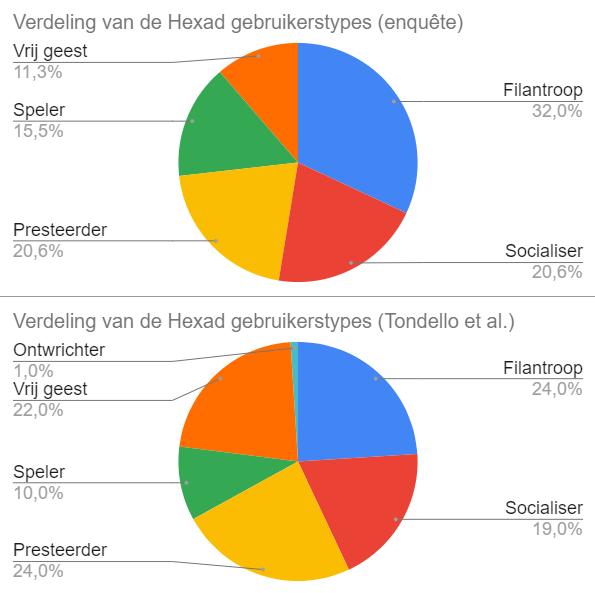
\includegraphics[width=\linewidth]{VergelijkingOnderzoek.png}
    \caption{Vergelijking van de verdeling van de gebruikerstypes.}
    \label{fig:vergelijkingonderzoek}
\end{figure}

De verdeling van de gebruikerstypes per geslacht is te zien in Figuur \ref{fig:verdelinggeslacht}. Hierin is te zien dat een groter aandeel van Filantropen, Socialisers en Presteerders te vinden is bij de vrouwen. Bij de mannen is dan weer een groter aantal Spelers en Vrije geesten te vinden. Via de onafhankelijkheidstoets werd nagegaan of een verband bestaat tussen de gebruikerstypes en het geslacht. Hierbij werd $\chi^2$(4) = 7.76 bekomen en p = 0.101. Dit resultaat toont dat geen significante associatie bestaat tussen de gebruikerstypes en het geslacht.

\begin{figure}
    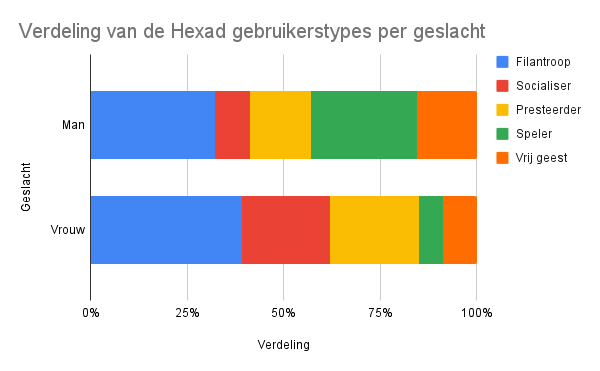
\includegraphics[width=\linewidth]{VerdelingGeslacht.png}
    \caption{Verdeling van de gebruikerstypes per geslacht.}
    \label{fig:verdelinggeslacht}
\end{figure}

In Figuur \ref{fig:verdelingleeftijd} is de verdeling van de gebruikerstypes bij elke leeftijdsgroep te zien. Hieruit blijkt dat hoe ouder een deelnemer is, hoe kleiner de kans is dat hij/zij een Speler is. De kans dat een deelnemer een Filantroop of Socialiser is neemt echter toe met de leeftijd. Met de onafhankelijkheidstoets werd nagegaan of een verband bestaat tussen de gebruikerstypes en de leeftijd. Voor $\chi^2$(24) werd 18.67 bekomen en voor p werd 0.770 bekomen. Hieruit kan geconcludeerd worden dat geen significant verband bestaat tussen de gebruikerstypes en de leeftijd.

\begin{figure}
    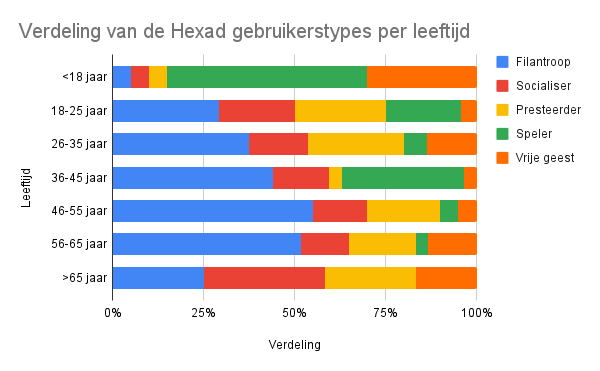
\includegraphics[width=\linewidth]{VerdelingLeeftijd.png}
    \caption{Verdeling van de gebruikerstypes per leeftijd.}
    \label{fig:verdelingleeftijd}
\end{figure}

Zoals eerder al werd vermeld kwam het soms voor dat bij het toewijzen van de gebruikerstypes gelijke scores werden behaald. Van alle deelnemers haalden 18.2\% van hen een gelijke score bij twee gebruikerstypes, 4.5\% haalde een gelijke score bij zowel drie gebruikerstypes als vier gebruikerstypes en 1.5\% haalden een gelijke score bij vijf gebruikerstypes. Geen enkele van de deelnemers haalde een gelijke score bij alle zes de types. Dit wil dus zeggen dat in totaal 28.7\% van de deelnemers geen specifiek gebruikerstype kreeg toegewezen. Het is daarom dat ook werd gekeken naar de verdeling van de zogenaamde hybride gebruikerstypes.

Bij het onderzoek naar de verdeling van de hybride gebruikerstypes werden zowel de gelijke scores bepaald als het verschil tussen de twee hoogste scores. Hieruit bleek dat voor 27.3\% van de deelnemers het verschil tussen de hoogste en tweede hoogste score 1 punt bedraagt, voor 22.7\% bedraagt het verschil 2 punten en voor 10.6\% bedraagt het verschil 3 punten. In combinatie met het aantal gelijke scores wil dit zeggen dat voor 89.3\% van de deelnemers het verschil tussen de hoogste scores ten hoogste 3 punten bedraagt. Dit is een laag verschil en toont aan dat gebruikers niet enkel door hun hoogste score een gebruikerstype kunnen worden toegewezen. In Tabel \ref{tab:aandeelhybridetypes} is daarom het aantal deelnemers te zien bij elke combinatie van toegewezen gebruikerstypes met een maximum verschil in scores van 3.

\begin{table}
    \begin{center}
        \begin{tabular}{c|c|c|c|c|c}
            \multicolumn{5}{c|}{\textbf{Gebruikerstypen}} & \textbf{Percentage} (\%)\\
            \hline
            Filantroop & Socialiser & & & & 16,7\% \\
            \hline
            Filantroop & Presteerder & & & & 16,7\%\\
            \hline
            Filantroop & Vrije geest & & & & 9,1\%\\
            \hline
            Presteerder & Speler & & & & 9,1\%\\
            \hline
            Presteerder & Socialiser & & & & 6,1\%\\
            \hline
            Speler & Vrije geest & & & & 4,5\%\\
            \hline
            Filantroop & Socialiser & Vrije geest & & & 4,5\%\\
            \hline
            Presteerder & Vrije geest & & & & 3,0\%\\
            \hline
            Socialiser & Vrije geest & & & & 3,0\%\\
            \hline
            Filantroop & Presteerder & Socialiser & & & 3,0\%\\
            \hline
            Filantroop & Speler & & & & 1,5\%\\
            \hline
            Filantroop & Socialiser & Speler & & & 1,5\%\\
            \hline
            Filantroop & Presteerder & Vrije geest & & & 1,5\%\\
            \hline
            Filantroop & Presteerder & Speler & & & 1,5\%\\
            \hline
            Presteerder & Speler & Vrije geest & & & 1,5\%\\
            \hline
            Filantroop & Socialiser & Speler & Vrije geest & & 1,5\%\\
            \hline
            Presteerder & Socialiser & Speler & Vrije geest & & 1,5\%\\
            \hline
            Filantroop & Presteerder & Socialiser & Vrije geest & & 1,5\%\\
            \hline
            Filantroop & Presteerder & Speler & Socialiser & Vrije geest & 1,5\%\\
        \end{tabular}
    \end{center}
    \caption{Aandeel van de hybride gebruikerstypes.}
    \label{tab:aandeelhybridetypes}
\end{table}

Figuur \ref{fig:hybridegeslacht} toont de verdeling van de zes meeste voorkomende hybride gebruikerstypes per geslacht. Bij de vrouwen is te zien dat ze bestaan uit een groter aandeel Filantroop-Presteerders en Filantroop-Socialisers. Bij de mannen zijn dan weer meer Presteerder-Spelers en Speler-Vrije geesten te vinden. Het Filantroop-Presteerder hybride gebruikerstype is bij de mannen niet te vinden.

\begin{figure}
    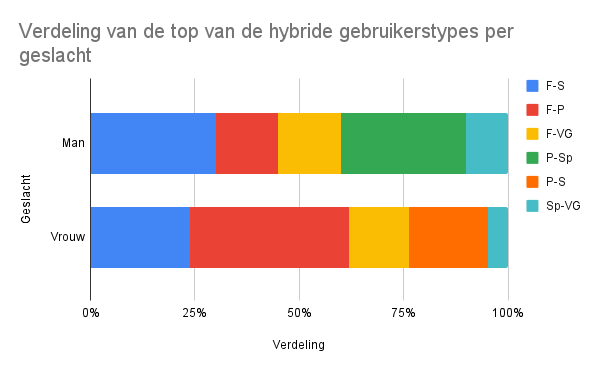
\includegraphics[width=\linewidth]{HybrideGeslacht.png}
    \caption{Verdeling van de top van de hybride gebruikerstypes per geslacht.}
    \label{fig:hybridegeslacht}
\end{figure}

In Figuur \ref{fig:hybrideleeftijd} is te zien dat het aandeel van de Filosoof-Socialisers en Filosoof-Presteerders met de leeftijd stijgt. Presteerder-Spelers en Speler-Vrije geesten zijn dan weer niet te vinden bij de oudere deelnemers.

\begin{figure}
    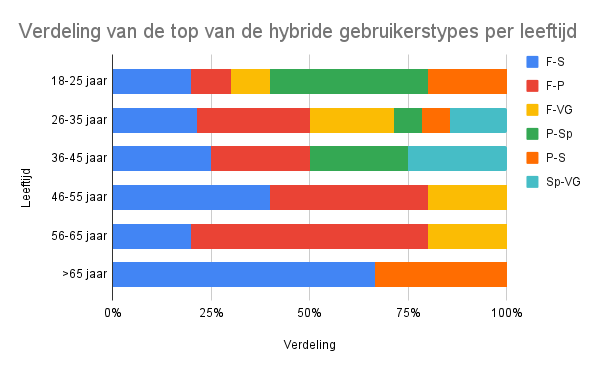
\includegraphics[width=\linewidth]{HybrideLeeftijd.png}
    \caption{Verdeling van de top van de hybride gebruikerstypes per leeftijd.}
    \label{fig:hybrideleeftijd}
\end{figure}

\textbf{Bespreking}



